\documentclass[../../main.tex]{subfiles}

% 

\begin{document}
\chapter{Rádioaktívne premeny jadier}
\section{Zadanie}

Základné zákony rádioaktívneho rozpadu, Aktivita, Postupný rozpad, Typy rádioaktívnych premien, Premena alfa, Premena beta, Kurieho diagram, Rozpadové schémy, Emisie žiarenia gama, Vnútorná konverzia elektrónov, Jadrové izomérie, Rádioaktívne rady, Transuránové prvky, Nuklidová karta, Výroba rádionuklidov.

\section{Rádioaktívne rady}
V dnešnej dobe poznáme 265 stabilných nuklidov, ostatné nuklidy sa samovoľne rozpadajú. To znamená, že sú rádioaktívne alebo sa spontánne štiepia. Rádioaktívne procesy prebiehajú teda bez vonkajšieho zásahu. Sú podmienené možnosťou prechodu z daného nestabilného systému do energetický nižšieho stavu, obecne nového systému. Strata energie jadra sa pritom deje buď emisiou častice alebo $\gamma$-žiarenia. Druh prechodu je určený energiou možných procesov a štruktúrou počiatočného a koncového stavu. Pokiaľ je ale energeticky možná emisia častice, je obyčajne uprednostňovaná.

Každý z troch klasických rádioaktívnych dejov je svojou fyzikálnou podstatou odlišný. Pri rozpade $\alpha$, ktorý je svojou povahou veľmi blízky štiepeniu, sa sformuje v jadre a vyžiari sa z neho častica $\alpha$, čiže jadro $_{2}^{4}$He. Rozpad $\beta$ je podmienený rozpadom neutrónu a jeho premenou na protón. A nakoniec rozpad $\gamma$, ktorého podstata spočíva v prechode jadra z vyššieho energetického stavu do nižšieho energetického stavu, pričom sa emituje fotón. Je to teda elektromagnetický prechod.  

Rozpadový rad je rad rádioaktívnych premien nestabilných izotopov, ktorý končí stabilným izotopom. Príklad takéhoto radu môžme vidieť na obrázku \ref{sf8:fig:rozpad}. Známe rádioaktívne rady, ktoré sú pomerne dosť dlhé, sú
\begin{itemize}
\item \textbf{thóriová} začínajúca nuklidom $_{90}^{232}$Th
\item \textbf{neptúniová} začínajúca nuklidom $_{93}^{237}$Np
\item \textbf{uránová} začínajúca nuklidom $_{92}^{238}$U
\item \textbf{aktiniová} začínajúca nuklidom $_{92}^{235}$U
\end{itemize}

Keďže pri $\alpha$ rozpade klesá neuklónové číslo $A$ o 4 a pri $\beta$ rozpade sa nemení, je možné rádioaktívny rozpad v danom rade charakterizovať zákonom udávajúcim veľkosť nukleónového čísla $A$ v danom rade
$$ A = 4n + D,$$
kde $n$ je celé číslo a $D=0$ pre thóriovú, $D=1$ pre neptúniovú, $D=2$ pre uránovú a $D=3$ pre aktiniovú radu. Konečné stabilné členy týchto radov sú niektoré izotopy olova $_{82}$Pb, u ktorého je protónové číslo $Z$ magickým, s výnimkou neptúniového radu, u ktorého je posledným nuklidom $_{83}^{209}$Bi, čo je najťažší známy stabilný nuklid. 

Niektoré rádionuklidy sa môžu rozpadať niekoľkými spôsobmi. Tento poznatok sa netýka len rádionuklidov, ktoré sú členmi rádioaktívnych radov. Príslušný jav sa nazýva vetvenie a relatívna pravdepodobnosť rôznych spôsobov rozpadu sa nazýva vetviaci pomer. Rádioaktívne jadrá charakterizujeme, spoločne s ďalšími obvyklými parametrami aj typom rádioaktívneho rozpadu, polčasom premeny, energiami vyžiarených častíc a spomenutými vetviacími pomermi.

\begin{figure}[!h]
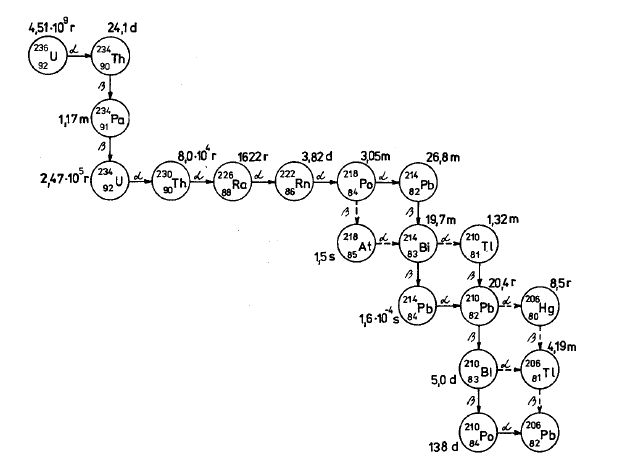
\includegraphics[width=0.9\textwidth]{subatom-08-rozpad.jpg}
\centering
\caption{Príklad rozpadového radu.}
\label{sf8:fig:rozpad}
\end{figure}

\section{Rádioaktívny zákon}
Empirický zákon rádioaktívneho rozpadu
\begin{equation}
N(t) = N(0)e^{-\lambda t},
\end{equation}
kde $N(0)$ je počiatočné množstvo atómov daného rádionuklidu, $N(t)$ je pravdepodobný počet nerozpadnutých atómov v čase $t$ a $\lambda$ je tzv. rozpadová konštanta, dostaneme riešením diferenciálnej rovnice pre úbytok počtu rádionuklidov s časom
\begin{equation}
-\frac{dN}{dt} = \lambda N . 
\end{equation}
Tento zákon sa dá odvodiť za dvoch predpokladov. Predpokladáme, že pravdepodobnosť rozpadu daného jadra je nezávislá na histórii tohto jadra a naviac táto pravdepodobnosť nie je ovplyvnená vonkajšími vplyvmi (ako napr. správanie susedných jadier v danej látke).

Na veličinu $N(t)$ je potrebné pozerať ako na pravdepodobnosť. Je to relatívna pravdepodobnosť toho, že v intervale $(0,t)$ nedôjde u daných jadier, ktorých bolo na začiatku $N(0)$, k rozpadu. $N(0)$ vyjadruje istotu, že všetky jadrá sú ešte v čase $t=0$ nerozpadnuté. Pravdepodobnosť, že častica prežije dobu $t$ a rozpadne sa v nasledujúcom infinitezimálnom časovom intervale ($t,t+dt$) je $dP(t)= \lambda e^{-\lambda t}dt$. Stredná doba života jadra $\tau$ bude daná integrálom
\begin{equation}
\tau = \int_0^{\infty} \lambda te^{-\lambda t}dt = \frac{1}{\lambda}.
\end{equation}
Narozdiel od strednej doby života je polčas rozpadu $T_{1/2}$ časom, za ktorý z pôvodného počtu jadier $N(0)$ ostane práve polovica. Z podmienky $N(T_{1/2}) = N(0)/2$ dostávame 
\begin{equation}
T_{1/2} = \frac{\ln2}{\lambda}.
\end{equation}
Zákon rádioaktívneho rozpadu je štatistický zákon. Preto počiatočný počet rádioaktívnych jadier $N(0)$ musí byť väčší než jedna, aby mal zmysel. Pokiaľ budeme mať len jedno jadro, potom $N(t)$ pre $t>0$ udáva len pravdepodobnosť, že v čase $t$ bude toto jadro ešte existovať. Veličina $\tau$ bude jeho stredná doba života. Jadro sa však môže rozpadnúť skôr alebo aj neskôr ako táto stredná doba života. Každý takýto individuálny proces je celkom náhodný. Ak ale budeme pozorovať dostatočne veľký súbor týchto individuálnych procesov u daného nuklidu, potom sa zmienené veličiny dajú ľahko merať a určovať. Problémy pri meraní nastávajú vtedy, keď sú stredné doby života veľmi krátke alebo príliš dlhé. V druhom prípade nám pomôže aktivita $A$ určiť potrebné konštanty rozpadu.

Aktivita je definovaná ako pravdepodobný počet premien (úbytok častíc) $dN$ za časový interval $(t,t+dt)$. Jednotkou aktivity je Becquerel (Bq). Platí pre ňu
\begin{equation}
A(t) = -\frac{dN}{dt} = \lambda N(t). 
\end{equation}
Môžme však aj definovať hmotnostnú, objemovú alebo plošnú aktivitu ako $A_m = A/m$, $A_V = A/V$ alebo $A_S = A/S$.
 
Ďalej sa zavádzajú veličiny ako absorbovaná dávka $D$, čo je pohltená energia žiarenia v danom prostredí. Udáva sa v jednotkách Gray $=$ J/kg. Zavádza sa aj tzv. dávkový ekvivalent $DE$, ktorý je daný vzťahom 
$$ DE = D Q_F,$$
kde $Q_F$ je tzv. quality factor udávaný v jednotkách Sievert (Sv). Jeho hodnoty pre rôzne druhy žiarenia sú v nasledujúcej tabuľke

\begin{figure}[!h]
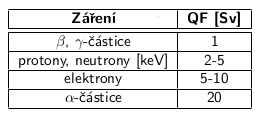
\includegraphics[width=0.4\textwidth]{subatom-08-tabul.png}
\centering
\label{sf8:fig:tabul}
\end{figure}

Pri emisii častíc a kvánt rádioaktívneho žiarenia dochádza vplyvom zákona zachovania hybnosti k spätnému odrazu jadra, ktoré preberá určitú malú časť kinetickej energie rozpadu. Tento jav sa prejavuje u každej rádioaktívnej premeny, najvýraznejšie však u rádioaktivity $\alpha$, lebo častice $\alpha$ majú vysokú hmotnosť a sú emitované s vysokou kinetickou energiou a hybnosťou. Spätný odraz môže viesť k uvoľneniu atómov z kryštálovej mriežky minerálu. Kinetická energia odrazených jadier sa nakoniec prejaví tepelnými účinkami.

V bežných jadrových aplikáciách sa žiadny spätný odraz prakticky neprejavuje. U niektorých presných spektroskopických meraniach však môže mať, spolu s tepelnými pohybmi atómov, výrazný vplyv. Príkladom je Mössbauerová spektroskopia alebo meranie presného tvaru spektra $\beta$-žiarenia za účelom stanovenia pokojovej hmotnosti neutrín.

Logický, avšak v bežných aplikáciách málo známy jav doprevádzajúci všetky druhy rádioaktivity je teplo. Pri rádioaktívnej premene vyletí z jadra s veľkou rýchlosťou častica (kvantum) žiarenia. Podľa zákona akcie a reakcie tým bude jadro (a vlastne i celý atóm) odhodené opačným smerom, bude mu teda udelená kinetická energie pohybu. Podobne pri absorpcii žiarenia v látke je predávaná energia na úrovni kinetickej energie atómu. Kinetická energia pohybu atómov v látke nie je nič iné než teplo. Pri každej ďalšej a ďalšej rádioaktívnej premene se takto budú viac a viac rozkmytávať atómy látky a teda rádioaktívna látka se bude zahrievať. Pri nízkych aktivitách používaných väčšinou v praxi je tento jav nepozorovateľný, avšak silné žiariče zahrievajú dosť silno (napríklad pri ožarovaní pri rádioterapii). Najsilnejšie žiariče sa musia dokonca chladiť, aby nedošlo k ich tepelnému poškodeniu.

Rádioaktívny rozpad je dej samovoľný. To znamená, že je spôsobený vnútornými mechanizmami stavby atómového jadra. Je nezávislý na vonkajších fyzikálnych a chemických vplyvoch a podmienkach (tlak, teplota, skupenstvo, vonkajšie pole atď.), Nedá sa ani urýchliť ani spomaliť. Jadro je skryté hlboko vo vnútri atómu, ktorého elektronový obal účinne odstraňuje všetky chemické, mechanické a teplotné vplyvy ako aj pôsobenie vonkajších polí.

Tento fakt ale nie je úplne absolútny a platí len za normálnych podmienok. Za extrémnych podmienok, napríklad zahriatím na veľmi vysokú teplotu, získavajú jadra takú vysokú kinetickú energiu, že prekonajú Coulombovskú odpudivú silu a môže tak teda dochádzať k jadrovým reakciám a zmenám rýchlosti a charakteru rádioaktívneho rozpadu. Štruktúru jadier, a tým aj rádioaktívny rozpad, je možné meniť ožarovaním pomocou neutrónov, urýchlených protónov či iných častíc, ktoré spôsobujú jadrové reakcie.

\paragraph{Postupný rozpad}
Pri postupnom rozpade sledujeme reťazový rozpad $A \rightarrow B \rightarrow C$, kde prvé dva rádionuklidy sú rádioaktívne a tretí je už stabilný. Majme teda pre každý rádionuklid v tomto reťazci zadané nasledovné veličiny

\begin{figure}[!h]
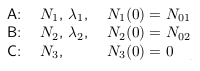
\includegraphics[width=0.3\textwidth]{subatom-08-cisla.png}
\centering
\end{figure}

Potom môžeme pre tento proces písať diferenciálnu rovnicu, ktorá popisuje rozpad nuklidu $A$ na nuklid $B$ a rozpad nuklidu $B$ na stabilný nuklid $C$

$$ \frac{dN_1}{dt} = -\lambda_1 N_1, $$
$$ \frac{dN_2}{dt} = \lambda_1 N_1 - \lambda_2 N_2, $$
$$ \frac{dN_3}{dt} = \lambda_2 N_2. $$

Po vyriešení sústavy diferenciálnych rovníc dostávame

$$ N_1(t) = N_{01}e^{-\lambda_1 t} $$

$$ N_2(t) = N_{02}e^{-\lambda_2 t} + N_{01}\frac{\lambda_1}{\lambda_2 - \lambda_1} \big( e^{-\lambda_1 t} - e^{-\lambda_2 t}  \big)$$

$$ N_3(t) = N_{02}(1-e^{\lambda_2t}) + N_{01}\frac{\lambda_1 \lambda_2}{\lambda_2 - \lambda_1} \bigg[ \frac{1}{\lambda_1}(1-e^{-\lambda_1t})   -\frac{1}{\lambda_2}(1-e^{-\lambda_2t}) \bigg] .$$

Je možné teda vidieť, že pomer $N_1$ a $N_2$ závisí iba od času ale aj od pomeru rozpadových konštánt. Pre všeobecné riešenie rozpadu $A_1 \rightarrow A_2 \rightarrow A_3 \rightarrow A_4 .... A_D$, kde $N_{01}\neq 0$ a ostatné $N_{0i}=0$, platí tzv. Batemanov zákon 

$$ N_D = \frac{N_1(0)}{\lambda_D} \sum_{i=1}^D \lambda_ic_ie^{-\lambda_it}, $$
kde
$$ c_i = \prod_{j=1, j\neq i}^D \frac{\lambda_j}{\lambda_j - \lambda_i} $$

\section{Rádioaktívna rovnováha}
Pod rádioaktívnou rovnováhou rozumieme situáciu, kedy množstvo jadier určitého rádionuklidu zostáva konštantné kvôli tomu lebo tieto rádioaktívne jadrá sú neustále doplňované nejakým produkčným mechanizmom. Týmto produkčným mechanizmom môžu byť jadrové reakcie (kozmogénne rádionuklidy, ktoré sú produkované neustále v atmosfére účinkom kozmického žiarenia) alebo rádioaktívny rozpad materského rádionuklidu na dcérske jadro, kde polčas rozpadu materského jadra bude podstatne dlhší než polčas rozpadu dcérskeho jadra.

Z časového hľadiska rozoznávame dva druhy rádioaktívnej rovnováhy
\begin{itemize}
\item Dlhodobá rovnováha, ktorá je zvaná tiež trvalá. Tento charakter majú už hore spomenuté kozmogénne rádionuklidy. V rozpadovom rádioaktívnom rade nastáva vtedy, keď materské jadro má oveľa dlhší polčas rozpadu než dcérske jadro. Vtedy z hľadiska časového horizontu polčasu rozpadu dcérskeho rádionuklidu môžeme jeho aktivitu považovať za konštantnú. Z dlhodobého hľadiska je trvalá rovnováha len približná, v skutočnosti rovnovážne množstvo dcérskeho rádionuklidu pomaly klesá s polčasom materského rádionuklidu. Trvalá rovnováha sa vyskytuje napríklad u $^{232}$Th, $^{235}$U a $^{238}$U.
\item Prechodová rovnováha nastáva vtedy, keď polčas rozpadu materského rádionuklidu je len o niečo dlhší než polčas rozpadu dcérskeho jadra. V nasledujúcom rozpade dvoch generačne viazaných rádionuklidov X, Y bude rýchlosť zmeny počtu jadier materského rádionuklidu X a dcérskeho rádionuklidu Y daná sústavou dvoch diferenciálnych rovníc

$$ \frac{dN_X}{dt} = \lambda_XN_X $$
$$ \frac{dN_Y}{dt} = \lambda_XN_X - \lambda_YN_Y $$

s okrajovými podmienkami $t=0:$ $NX(0)=N_{X0}$, $N_Y(0)=0$. Pre dcérsky rádionuklid potom dostávame rozpadový zákon v tvare

$$ N_Y(t) = N_{X0}\frac{\lambda_X}{\lambda_Y - \lambda_X} (e^{-\lambda_Xt}-e^{-\lambda_Yt}).$$

Pre materský rádionuklid X zostáva klasický mono-exponenciálny zákon

$$ N_X(t) = N_{X0}e^{-\lambda_Xt}.$$

Pokiaľ je $\lambda_X<\lambda_Y$, potom po dostatočne dlhom čase je exponenciálny člen $e^{-\lambda_Yt}$ zanedbateľne malý v porovnaní s členom $e^{-\lambda_Xt}$. Rozpadový zákon pre dcérsky rádionuklid sa potom zjednoduší na nasledujúci tvar

$$ N_Y(t) = N_{X0}\frac{\lambda_X}{\lambda_Y - \lambda_X}e^{-\lambda_Xt} = N_X(t)\frac{\lambda_X}{\lambda_Y - \lambda_X} $$

Po dostatočne dlhom čase sa ustáli rovnovážny pomer medzi dcérskym a materským rádionuklidom - prechodná rovnováha. Pri tejto rovnováhe aktivita dcérskeho rádionukllidu klesá s polčasom materského rádionuklidu. Aktivita dcérskeho rádionuklidu 

$$ A_Y(t) = \lambda_YN_Y = N_X(t)\frac{\lambda_X\lambda_Y}{\lambda_Y-\lambda_X} $$

sa pritom udržuje vyššia než okamžitá aktivita materského rádionuklidu.

Pokiaľ je $\lambda_X\ll\lambda_Y$, tak pre časy krátke, v porovnaní s polčasom rozpadu rádionuklidu X, je $\lambda_X \ll 1$ a prvý exponenciálny člen $e^{-\lambda_Xt}$ môžme aproximovať jednotkou. Po uplynutí niekoľkých polčasov rozpadu dcérskeho rádionuklidu Y (keď druhý exponenciálny člen je blízky nule) sa ustáli rovnovážne množstvo tohto rádionuklidu na 

$$ N_Y = \frac{\lambda_Y}{\lambda_X}N_X, $$ 

tj. trvalá rovnováha. Jeho rovnovážna aktivita 

$$ A_Y = \lambda_YN_Y = \lambda_XN_X = A_X $$

bude rovná aktivite materského rádionuklidu $X$. Z dlhodobého hľadiska aj toto rovnovážne množstvo klesá s polčasom rozpadu materského rádionuklidu $X$.
\end{itemize}

Trvalá a prechodová rovnováha sú ilustrované na obrázku \ref{sf8:fig:dec}, kde je zobrazená aktivita rádionuklidu v závislosti na čase 
\begin{figure}[!h]
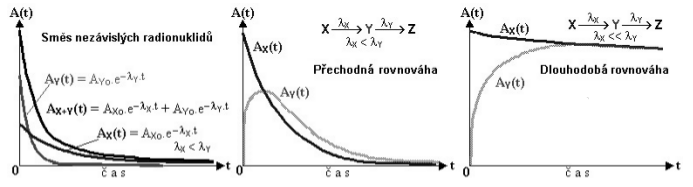
\includegraphics[width=1.0\textwidth]{subatom-08-dec.png}
\centering
\caption{Aktivita materských a dcérskych rádionuklidov v závislosti na čase.}
\label{sf8:fig:dec}
\end{figure}

\section{Tvorba rádionuklidov}
Rádionuklidy možno vytvárať ožarovaním stabilných prvkov v reaktore alebo na urýchľovači. Ak máme doštičku s objemom $V=Sd$, kde $S$ je jej plocha a $d$ je jej hrúbka, v ktorej sa nachádza $n$ častíc stabilného prvku, potom počet vytvorených častíc za jednotku času je 
$$ q = \phi Vn \sigma,$$
kde $\sigma$ je účinný prierez reakcie a $\phi$ je tok častíc. Potom zmena počtu častíc v doštičke za jednotku času je daná diferenciálnou rovnicou
$$ \frac{dN}{dt} = q - \lambda N, $$
ktorej riešenie je 
$$ N(t) = \frac{q}{\lambda} (1-e^{-\lambda t}).$$
Tento výsledok svedčí o tom, že pri ožarovaní rastie počet rádionuklidov až k hodnote $N=q / \lambda$, a po skončení ožarovania tento počet začne exponenciálne klesať, viď obrázok \ref{sf8:fig:tvorba}.

\begin{figure}[!h]
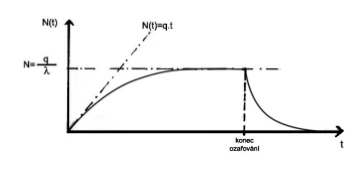
\includegraphics[width=0.5\textwidth]{subatom-08-tvorba.png}
\centering
\caption{Počet rádionuklidov v závislosti na čase.}
\label{sf8:fig:tvorba}
\end{figure}

\section{Rozpad $\alpha$}
Ešte predtým, než sa začneme zaoberať alfa rozpadom, je potrebné spomenúť, že sa jedná o veľmi asymetrický rozpad atómového jadra. Pri tomto procese totiž atómové jadro emituje jadro $_{2}^4$He, ktorého konštituenty sú viazané silnou interakciou. Avšak, nukleóny v $_{6}^{12}$C sú viazané ešte silnejšie a preto v niektorých ťažkých jadrách existuje pravdepodobnosť pre rozpad emitovaním $_{6}^{12}$C. Rovnako tak isto bol objavený rozpad emisiou $_{6}^{14}$C, k nemu však dochádza veľmi zriedka. Ďalšie podobné rozpady sú predmetom skúmania. Takéto procesy tvoria spektrum všetkých možností, ktorými sa môže ťažké jadro rozpadnúť na dve (alebo viac) častí. Na jednom konci spektra je výsledkom rozpadu jedno ľahké jadro a jedno ťažké, na druhom konci spektra sú dve približne rovnako hmotné atómové jadrá (spontánne štiepenie).
Rozpad emisiou alfa častice tak možno nazvať veľmi asymetrickým štiepením.

Veľa ťažkých jadier, ako napríklad urán alebo rádium, sa spontánne rozpadá emisiou $\alpha$-častice. Spontánny rozpad atómového jadra, pri ktorom je vyžiarená $\alpha$-častice, sa schematicky zapisuje ako
$$ _Z^AX \rightarrow _{Z-2}^{A-4}X + _2^4He, $$
kde na ľavej strane je tzv. materské jadro $_Z^AX$ s daným počtom nukleónov a protónov a na pravej strane prvý člen reprezentuje tzv. dcérske jadro a druhý člen je $\alpha$ častica. Často sa stáva, že i dcérske jadro je rádioaktívne, vďaka čomu potom sledujeme rádioaktívne rozpadové rady.

Uvažujme hodnotu uvoľnenej energie $Q$ pre $\alpha$ rozpad jadra $A(Z,N)$. Tá je daná ako rozdiel súčtu väzbových energii produktov rozpadu a väzbovej energie rozpadajúceho sa jadra (pritom používame definíciu väzbovej energie z kvapkového modelu, Bethe-Weizsäckerovu formulu)

$$ Q = B(Z-2, A-4)+B(2,4)-B(Z,A) $$

alebo ju môžme definovať ako 

$$ Q = \big[ m(X)-m(Y)-m(^4_2He) \big] = T_{\alpha} + T_Y, $$

kde $T$ označuje kinetickú energiu častice. K $\alpha$ rozpadu môže dôjsť, keď $Q>0$, tj. pokiaľ

$$ B(2,4) > B(Z,A)-B(Z-2,A-4) \approx 4\frac{dB}{dA} = 4 \bigg[ A \frac{d(B/A)}{dA}+\frac{B}{A} \bigg].$$

Pre jadra s $A>120$ je $\frac{d(B/A)}{dA} \approx -7.7\times10^{-3}$, a keďže väzbová energia $\alpha$ častice je $B(2,4)\approx 28.3\,MeV$,
môže byť nerovnosť splnená, pokiaľ 
$$\frac{B}{A}\leq 7.075\,MeV + 7.7\times 10^{-3}A ,$$
čo platí pre $A>140$. Tieto jadra sú teda nestabilné voči $\alpha$ rozpadu.

Uvoľnená energia $Q$ sa z časti využije ako excitačná energia dcérskeho jadra $R_{exc}$ a z časti ako kinetická energia $\alpha$ častice a dcérskeho jadra
$$ Q = E_{exc}+T_{\alpha}+T_Y .$$
Kinetická energia $\alpha$ častice nikdy nie je presne rovná energii rozpadu $Q$, pretože v dôsledku zákona zachovania hybnosti jadro pri emisii $\alpha$ častice odskakuje s malou kinetickou energiou. Ľahko sa dá ukázať, že ako dôsledok zachovania hybnosti a energie súvisí $T_{\alpha}$
s $Q$ a s nukleónovým číslom $A$ pôvodného jadra vzťahom\footnote{Pokiaľ je materské jadro pred rozpadom v kľude, potom dcérske jadro a $\alpha$ častica budú po rozpade mať rovnako veľké ale opačné hybnosti $p$. Energiu rozpadu $Q$ potom môžme vyjadriť ako $$ Q=T_Y+T_{\alpha}=\frac{p^2}{2m_Y}+\frac{p^2}{2m_{\alpha}}= \frac{p^2}{2m_{\alpha}}\bigg(1 + \frac{m_{\alpha}}{m_Y} \bigg), $$ 
následne použitím vzťahu $T_{\alpha} = \frac{p^2}{2m_{\alpha}}$ a $\frac{m(\alpha)}{m(Y)}= \frac{4}{A-4}$ dostávame vzťah \ref{sf8:rovnica1}.} 

\begin{equation}
T_{\alpha} = \frac{A-4}{A}Q.
\label{sf8:rovnica1}
\end{equation}

Hmotnostné číslo takmer všetkých žiaričov $\alpha$ je vyššie než 210, a tak sa väčšina rozpadovej energie prejavuje ako kinetická energia $\alpha$ častice. Napríklad pri rozpade $_{86}$Rn je $Q = 5.57\,\unit{MeV}$ a $T_{\alpha}  = 5.486\,\unit{MeV}.$ Naviac pre ťažké atómové jadrá približne platí $T_Y\approx 0.02Q.$

Kinetická energia $\alpha$ častice vykazuje isté pravidelnosti, viď obrázok \ref{sf8:fig:alfa} - pomaly a nie monotónne rastie s nukleonovým číslom $A$. U izotopov daného prvku klesá s rastúcim číslom A s výnimkou úzkej oblasti u magického čísla $N=126$. Z obrázka aj z ďalších dát je zrejmé, že energia $\alpha$ častice leží v intervale $(3;9)\,\unit{MeV}$. Nie je však nevyhnutné, aby dcérske jadro vzniklo v základnom stave a preto spektrum energie častíc $\alpha$ nie je všeobecne reprezentované jediným bodom ale má jemnú štruktúru a skladá sa z niekoľkých ostrých hodnôt energie. 

\begin{figure}[!h]
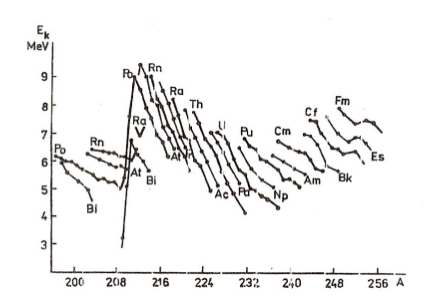
\includegraphics[width=0.5\textwidth]{subatom-08-alfa.png}
\centering
\caption{Závislosť kinetickej energie $T_{\alpha}$ vyžarovaných $\alpha$ častíc na nukleónovom čísle A.}
\label{sf8:fig:alfa}
\end{figure}

Pokiaľ sa všetky $\alpha$ rozpady prihodia medzi základným stavom materského jadra a základným stavom dcérskeho jadra, potom budú mať všetky emitované $\alpha$ častice tú istú kinetickú energiu, ktorú možno spočítať z celkovej energie rozpadu $Q$ vzťahom (\ref{sf8:rovnica1}). Keď ale meriame energie emitovaných $\alpha$ častíc s vysokým rozlíšením možno pozorovať isté energetické spektrum, ako je to naznačené v rozpade $^{227}$Th na $^{223}$Ra na obrázku \ref{sf8:fig:alfaspectrum}.

\begin{figure}[!h]
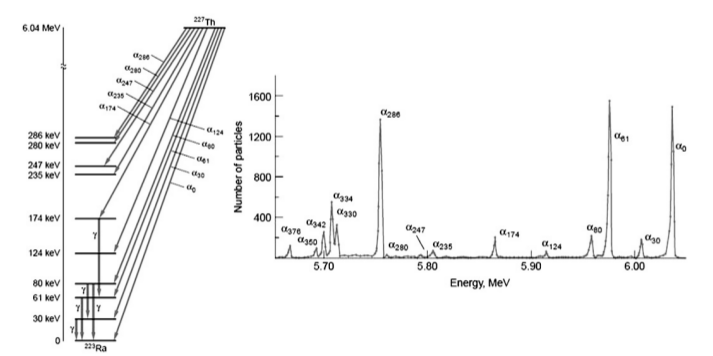
\includegraphics[width=1.0\textwidth]{subatom-08-alfaspectrum.png}
\centering
\caption{Vľavo vidíme energetické stavy $^{223}$Ra určené meraním energie $\alpha$ častíc z $^{227}$Th. Vpravo vidíme energetické spektrum $\alpha$ častíc z $^{227}$Th. Najenergetickejšie $\alpha$ častice odpovedajú prechodom do základného stavu $^{223}$Ra s energiou rozpadu, ktorú v texte označujeme ako $Q$. Meraním $\alpha$ častíc sa dajú určiť energetické stavy dcérskeho jadra $^{223}$Ra.}
\label{sf8:fig:alfaspectrum}
\end{figure}

Významnou charakteristikou rozpadu $\alpha$ sú stredné doby života ($\tau$) jadier podliehajúcich tomuto rozpadu. Sú síce pre daný typ nuklidu nemenné, avšak pre rôzne jadra ležia v ohromnom intervale $(10^{-7}-10^{25}\,\unit{s})$. V nasledujúcej tabuľke je niekoľko príkladov

\begin{figure}[!h]
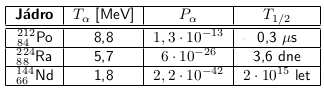
\includegraphics[width=0.4\textwidth]{subatom-08-alfatab.png}
\centering
\caption{Kinetická energia alfa častice, pravdepodobnosť pretunelovania potenciálovou bariérou a polčas rozpadu pre niekoľko jadier, ktoré podliehajú alfa rozpadu.}
\label{sf8:fig:alfatab}
\end{figure}

Vzťah medzi rozpadovou konštantou $\lambda$ a doletom $R$ častice $\alpha$ je pomerne dlho známy. Platí preň empirické pravidlo nájdené pri štúdiu rádioaktívnych radov. Jeho tvar je nasledovný
$$ \ln \lambda = A \ln R + B, $$
kde $A$ a $B$ sú konštanty. Vzhľadom k tomu, že poznáme empirický vzťah medzi doletom $R$ a energiou a že je $\lambda = 1 / \tau$, poskytuje spomínaná relácia možnosť odvodiť empirický vzťah medzi energiou vyžiarenej častice a strednej doby života materského jadra.

Žiarenie $\alpha$ vďaka svojmu dvojnásobnému kladnému náboju pri vniknutí do látky veľmi účinne vytrháva elektróny z obalov atómov, čím rýchlo stráca energiu a pri bežných energiách sa zabrzdí asi po $0,1\,\unit{mm}$ v látkach hustých ako voda alebo tkanivo. Vďaka tejto malej prenikavosti ho nemožno využiť v diagnostike ani v terapii. Využíva sa len sporadicky v niektorých detekčných zariadeniach (napríklad detektory hustoty plynov, požiarne hlásiče) alebo v neutrónových generátoroch.

Teraz však už pristúpme k samotnému mechanizmu $\alpha$-rozpadu. Predpokladáme, že častica $\alpha$ existuje predpripravená vo vnútri ťažkého jadra. Takáto častica sa neustále pohybuje a je v jadre udržovaná potenciálovou bariérou, ktorá ju obklopuje. Aby sa ale dostala z jadra von, musí pretunelovať Coulombovskou bariérou, čo je možné s pravdepodobnosťou, ktorá je malá, avšak nenulová. Táto nenulová pravdepodobnosť pretunelovania bariérou existuje zakaždým, keď častica narazí na danú bariéru. Avšak energia tejto častice musí byť na úrovni niekoľko MeV. Keďže je táto energia menšia ako energia bariéry, pri prechode častice bariérou sa vlnová funkcia častice $\alpha$ zmenší exponenciálne, viď obrázok \ref{sf8:fig:beriera}. Pravdepodobnosť emisie častice $\alpha$ je tak veľmi citlivá funkcia jej energie, čo vysvetľuje obrovský rozsah polčasov rozpadu, ktoré boli nájdené experimentálne.

Výpočet rozpadovej konštanty $\lambda$ znamenal prvú úspešnú aplikáciu kvantovej mechaniky na atómové jadro. Rozpadová konštanta je súčinom pravdepodobnosti $\lambda_0$ - že sa $\alpha$-častica sformuje v atómovom jadre blízko jeho povrchu, a koeficientu prieniku bariérou $P_{\alpha}$

$$ \lambda = \lambda_0 P_{\alpha}. $$

Člen $\lambda_0$ by mal zahŕňať faktor, ktorý udáva pravdepodobnosť nájdenia $\alpha$-častice v jadre a faktor, ktorý reprezentuje počet pokusov $\alpha$-častice o prienik bariérou za jednu sekundu. Približný odhad tohto druhého faktora je $v_0/2R$, kde $v_0$ je rýchlosť častice a $2R$ je priemer častice.

\begin{figure}[!h]
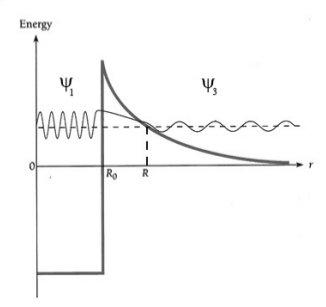
\includegraphics[width=0.4\textwidth]{subatom-08-bariera.png}
\centering
\caption{Prienik $\alpha$-častice potenciálovou bariérou.}
\label{sf8:fig:beriera}
\end{figure}

Koeficient prieniku bariérou je daný pomerom medzi tokom, ktorý je prenesený cez bariéru a prichádzajúcim tokom. Pre jedno-dimenzionálnu bariéru môžme použiť WKB aproximáciu a koeficient prieniku vyjadriť v tvare

$$ P_{\alpha} = \bigg\vert \frac{\psi_3}{\psi_1} \bigg\vert^2 \approx e^G = \exp \bigg[ -\frac{2}{\hbar} \int_{R_0}^R \sqrt{2m[V(r)-E]}dr  \bigg],$$
kde $R_0$ a $R$ sú klasické body obratu častice, 
$$ V(r)=\frac{1}{4\pi \epsilon_0} \frac{Z_1 Z_2 e^2}{r} $$
je Coulombický potenciál a $G$ je Gamow súčiniteľ prieniku. Tento koeficient prieniku je veľmi citlivý na výšku ale aj šírku bariéry. 

\begin{itemize}
\item Na vzdialenostiach menších než $R_0$, čo aproximuje rozmer jadra, je alfa častica v potenciálovej jame nešpecifikovanej hĺbky, ktorá reprezentuje účinok jadrovej väzbovej sily na alfa časticu. 
\item Na vzdialenosti $R_0$ sa tento potenciál stane kladným a nadobúda svoje maximálne hodnoty
$$ V(R_0) = \frac{zZe^2}{4\pi \epsilon_0 R_0}, $$ 
kde $z=2$ a $Z$ je protónové číslo zbytku jadra. 
\item Na vzdialenostiach väčších ako $R_0$ je potenciál Coulombovský.
\end{itemize}

\section{Rozpad $\beta$}
Rozpad $\beta$ je rádioaktívny proces, v ktorom jadro emituje elektrón ($\beta^-$ rozpad) alebo pozitrón ($\beta^+$ rozpad) a transformuje sa tým na izobary s nábojom $Z\pm1$. Môžeme poznamenať, že rozpad $\beta$ je troj-časticový rozpad narozdiel od $\alpha$ rozpadu, ktorý je dvoj-časticový. Podobná transformácia sa deje aj záchytom elektrónu, pri ktorom je v jadre zachytený atómový elektrón. $\beta^-$ rozpad bol jedným z prvých pozorovaných rádioaktívnych procesov, $\beta^+$ rozpad bol pozorovaný v roku 1934 a elektrónový záchyt v roku 1938.

Skúmanie rádioaktivity $\beta$ prinieslo oveľa viac prekvapujúcich poznatkov než štúdium rádioaktivity $\alpha$. Pri $\beta$ rozpade sa fyzika prvýkrát bezprostredne zoznámila s novým typom interakcie, s interakciou slabou, ktorá sa líši od interakcie elektromagnetickej, silnej a gravitačnej.

Otázkou tiež bolo, či elektrón, ktorý je emitovaný z jadra, môže existovať v tomto jadre. Podľa Heisenbergovho princípu neurčitosti, ktorý spája stredné kvadratické odchýlky polohy a hybnosti častice, by stredná kvadratická odchýlka hybnosti elektrónu v jadre (ak za strednú kvadratickú odchýlku polohy dosadíme priemer jadra) bola $\approx 20 MeV$, čo je dosť na to, aby elektrón mohol z jadra uniknúť. Zo štruktúry jadra ale vieme, že elektrón sa v jadre vyskytovať nemôže. Preto môžme tvrdiť, že elektrón je v jadre vytvorený v čase rozpadu. Jednotlivé procesy sú teda

\begin{itemize}
\item $\beta^{-}$ rozpad: $ n \rightarrow p + e^{-} + \bar{\nu}_e$
\item $\beta^{+}$ rozpad: $ p \rightarrow n + e^{+} + \nu_e$
\item Elektrónový záchyt: $ p + e^{-} \rightarrow n + \nu_{e} $ 
\end{itemize}

Všetky tri procesy, ktoré zahŕňame do rádioaktivity $\beta$, majú spoločný základ v nestabilite nukleónu. Vieme, že voľný neutrón má pokojovú hmotnosť, a teda aj pokojovú energiu väčšiu, než je pokojová hmotnosť či pokojová energia protónu. To mu dovoľuje rozpadnúť sa $\beta^-$ rozpadom so strednou dobou života 896 sekúnd. Zo zákona zachovania energie vyplýva, že voľný protón sa nemôže rozpadnúť na neutrón a ďalšie častice. Ale protón viazaný v jadre na dostatočne vysokej hladine môže prejsť na voľnú neutrónovú hladinu v jadre. Táto neutrónová hladina ale musí ležať nižšie než je hladina, na ktorej sa protón nachádza. V takom prípade môže nastať $\beta^+$ rozpad. Za rovnakých podmienok môže protón zachytiť elektrón z K vrstvy a stať sa neutrónom.

Ak by sme v spomínaných procesoch neuvažovali neutríno, stretli by sme sa s niekoľkými vážnymi problémami. Keďže neutrón, protón aj elektrón sú častice so spinom 1/2, bol by $\beta^-$ a $\beta^+$ rozpad zakázaný, pretože nie je možné, aby dve častice so spinom 1/2 dali tretiu časticu, ktorá by opäť mala spin 1/2. Ďalej by sme nemohli vysvetliť energetické spektrum elektrónov, ktoré je spojité, zatiaľčo procesy bez neutrína by predstavovali dvoj-telesový rozpad, ktorý má diskrétne spektrum.

Aby sa vyriešili tieto ťažkostí navrhol Wolfgang Pauli v roku 1931 ideu, že sa v $\beta$ rozpade emituje ďalšia častica - neskôr nazvaná neutríno. Tá by mala mať nulovú hmotnosť, spin 1/2 a mala by byť bez náboja. Keďže elektróny a neutrína sú leptóny, musí v reakcii platiť aj zákon zachovania leptonového čísla.

Ďalej zavedieme energetické podmienky pre beta rozpad
\begin{figure}[!h]
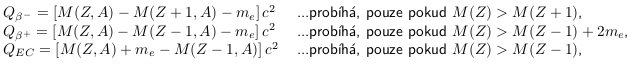
\includegraphics[width=0.9\textwidth]{subatom-08-beta.png}
\centering
\end{figure}

kde $M(Z)$ je hmotnosť atómov a nie len jadra. Prechody sú možné len vtedy, keď celková energia uvoľnená v rozpade je nezáporná, teda $Q\geq0$. Z energetickej bilancie je naviac zrejmých niekoľko faktov. Elektrónový záchyt (EZ) a $\beta^+$ rozpad sú konkurenčné procesy, pričom EZ je energeticky výhodnejší, lebo
$$ Q_{EZ} = Q_{\beta^+}+2m_{e}c^2.$$

Vyžiarenie pozitrónu v $\beta^+$ rozpade je možné jedine vtedy, ak je rozdiel pokojových energii materského a dcérskeho atómu väčší ako $2m_ec^2$. Vďaka tomu, že $\beta^+$ rozpad a elektrónový záchyt vedú k rovnakému výslednému atómovému jadru, obidva javy si navzájom konkurujú. Ak  $Q_{EZ} $ patrí do intervalu $(0,2m_ec^2),$ potom je možný len elektrónový záchyt. Názorne môžme konkurenciu oboch procesov pozorovať na obrázku \ref{sf8:fig:betarozpad}.

\begin{figure}[!h]
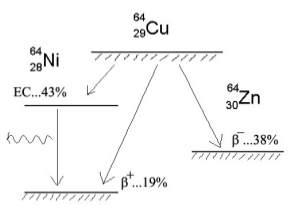
\includegraphics[width=0.4\textwidth]{subatom-08-betarozpad.png}
\centering
\caption{Energetický diagram prechodu $^{64}_{29}Cu$.}
\label{sf8:fig:betarozpad}
\end{figure}

Keďže pri elektrónovom záchyte je emitované iba neutríno, zdalo by sa, že je takmer nemožné túto reakciu pozorovať (vieme o obtiažnosti, ktoré sprevádzajú detekciu neutrín). Záchyt elektrónu (najčastejšie sa jedná o elektrón z K vrstvy, s oveľa menšou pravdepodobnosťou je možné aj záchyt elektrónu z L vrstvy) ale necháva v atómovom obale vakanciu (voľné miesto), ktorá je zaplnená ďalším atómovým elektrónom z vyššej vrstvy, vďaka čomu je emitované charakteristické gama žiarenie alebo Augerov elektrón. Tieto komponenty už možno ľahko detekovať.

Ako už bolo uvedené, spektrum kinetickej energie elektrónov je spojité. Maximálna energia vyžiarených elektrónov pri $\beta$ rozpade sa pohybuje v intervale od $0,02\,\unit{MeV}$ u trícia ($^3_1$H) až po $13,4\,\unit{MeV}$ u bóru ($^{12}_{5}$B).

Beta rozpadu podliehajú izotopy veľmi ľahkých jadier ale aj nestabilné izotopy stredne ťažkých a najťažších jadier. Najľahším známym rádioizotopom, ktorý podlieha beta rozpadu je trícium ($^3_1$H), najťažším einsteinium ($^{255}_{99}$Es). Pri ťažších nestabilných jadrách začína s rastúcim protónovým číslom $Z$ prevládať konkurenčný alfa rozpad ale aj iné typy rozpadu.

\section{Fermiho teória beta rozpadu}
Zo všeobecných vlastností beta rozpadu je zrejmé, že za proces je zodpovedná nová interakcia. Kdekoľvek sa odohráva táto interakcia medzi hadrónom a leptónom, vždy je zahrnuté neutríno či antineutríno. Navyše aj polčasy beta rozpadu sa dosť odlišujú. Nadobúdajú totiž hodnoty od zlomok sekúnd až po mnoho rokov, čo indikuje, že ona nová interakcia musí byť slabšia ako silná a elektromagnetická interakcia. Odtiaľ pre ňu plynie názov slabá interakcia.

Teória beta rozpadu bola vyvinutá Enricom Fermim v roku 1934 použitím Fermiho zlatého pravidla pre rozpadovú konštantu
$$ \lambda = \frac{2\pi}{\hbar}\vert V_{fi} \vert^2 \rho, $$
kde $V_{fi} = \int \psi^{*}_f V \psi_i d\tau$ je maticový element a $\rho = dn/dE_f$ je hustota koncových stavov s energiou $E_f$.

Pôvodne nebolo o operátore $V_{fi}$ známe nič, až na to, že musí spĺňať určité všeobecné transformačné pravidlá. Ďalšie skúmanie ukázalo, že proces beta rozpadu môže mať buď vektorový charakter (Fermiho prechod, kedy zmena spinu je $\Delta I = 0$ a spiny sú orientované anti-paralelne) alebo axiálne-vektorový charakter (Gamow-Tellerov prechod, zmena spinu je $\Delta I = 0,1$ a spiny sú orientované paralelne). Napíšeme maticový element $V_{fi}$ pomocou faktoru $g$, ktorý reprezentuje silu interakcie, a operátora $O_x$ reprezentujúceho formálne vlastnosti interakcie, ktorá musí zachovávať priestorové a spinové symetrie rozpadových produktov, teda

$$ V_{fi} = g \int \psi^{*}_f O_x \psi_i d\tau. $$

Teraz môžme zhrnúť teóriu beta rozpadu (s modifikáciami možno aplikovať aj na elektrónový záchyt). Vlnová funkcia koncového stavu je daná súčinom funkcie $\chi_f$, ktorá reprezentuje stav jadra po rozpade, a vlnových funkcii $\varphi_e$ a $\varphi_{\nu_e}$, ktoré popisujú relatívny pohyb elektrónu a neutrína. Spinové funkcie teraz nezahrňujeme. Vlnové funkcie elektrónu a neutrína s hybnosťou $\vec{p}$, resp. $\vec{q}$ možno vyjadriť ako rovinné vlny normalizované k objemu $V$
$$ \varphi_e = \frac{1}{\sqrt{V}}e^{i\vec{p}\cdot \vec{r}/\hbar}  \hspace{1cm}  \varphi_{\nu_e} = \frac{1}{\sqrt{V}}e^{i\vec{q}\cdot \vec{r}/\hbar}. $$

Použitie rovinnej vlny na opis neutrína je oprávnený, pretože neutríno neinteraguje silno s ostatnými časticami. Avšak z dôvodu interakcie elektrónu s Coulombovským poľom je aproximácia jeho pohybu rovinnou vlnou správna len pri vysokých energiách elektrónu.

Keďže pre energie pri beta rozpade sú exponenty vo vyššie uvedených vlnových funkcií ďaleko menšie ako jedna, možno vziať do úvahy len niekoľko prvých členov Taylorovho rozvoja
$$ e^{i\vec{p}\cdot \vec{r}/\hbar} = 1+ \frac{i\vec{p}\cdot\vec{r}}{\hbar} +...$$
$$ e^{i\vec{q}\cdot \vec{r}/\hbar} = 1+ \frac{i\vec{q}\cdot\vec{r}}{\hbar} +...$$

Pokiaľ budeme brať len konštantné členy, maticový element $V_{fi}$ prejde v
$$ V_{fi}=\frac{q}{V} \int \chi_f^{*}O_x\chi_i d\tau = \frac{q}{V}M-{fi},$$
kde $\chi_f$ a $\chi_i$ sú vlnové funkcie koncového a počiatočného stavu jadra a $M_{fi}$ je jadrový maticový element, ktorý neobsahuje žiadnu závislosť na energii elektrónu či neutrína. Toto priblíženie zodpovedá tomu, čo sa nazýva dovolený beta rozpad. V tomto prípade je všetká závislosť rozpadovej konštanty na energii schovaná v člene $\rho$, ktorý reprezentuje počet koncových stavov dostupných pre rozpadové produkty.

Celková energia systému je daná s nepresnosťou $\Delta E$, ktorá odpovedá prirodzenej šírke počiatočného stavu. Ak uvážime prechod do určitého stavu jadra, potom koncové stavy sú len tie, kde celková energia voľných leptónov má tú istú neurčitosť.

Aby sme určili spektrum energií emitovaných elektrónov, je potrebné vyčísliť parciálnu rozpadovú konštantu $d\lambda$, ktorá odpovedá emisii elektrónov s hybnosťou v intervale ($p,p+dp$). To je možné urobiť tak, že priradíme elektrónu hybnosť $p$ a zadefinujeme $\lambda$ ako odpovedajúcu rozpadovú konštantu. Potom vezmeme do úvahy, že experimentálna aparatúra určuje počet elektrónov, ktoré majú hybnosť v danom intervale, a definujeme parciálnu rozpadovú konštantu $d\lambda$ ako
$$ d\lambda = \lambda_p \frac{dn}{dp}dp, $$
načo vyintegrujeme cez všetky možné hybnosti, aby sme dostali celkovú rozpadovú konštantu
$$ \lambda = \int \lambda_p \frac{dn}{dp}dp. $$
Rozpadová konštanta $\lambda_p$ je určená zlatým Fermiho pravidlom s hustotou rozpadových stavov $\rho = dn/dE_{f}$. Ak vezmeme do úvahy reláciu medzi energiou neutrína a elektrónu a zanedbáme pritom veľmi malú kinetickú energiu jadra, dostaneme
$$ E_f = E_e + E_{\nu_e} = m_ec^2 + T_e +T_{\nu_e} = m_ec^2+Q.$$
Ak budeme predpokladať, že neutríno má nulovú hmotnosť, potom platí pre jeho energiu $E_{\nu_e} = qc$, čo po dosadení do vzťahu vyššie dáva 
$$ q = \frac{Q-T_e}{c}, $$
kde $c$ je rýchlosť svetla. Takže pre fixovanú energiu elektrónu je $dE_f=cdq$ a pre hustotu finálnych stavov dostávame
$$ \frac{dn}{dE_f} = \frac{dn}{dq}\frac{dq}{dE_f} = \frac{dn}{dq}\frac{1}{c}.$$
Konečnou zámenou $\lambda_p$ za $\lambda$ vo Fermiho zlatom pravidle a dosadením za $\rho(E_f)$ môžme písať pre parciálnu rozpadovú konštantu
$$ d\lambda = \frac{2\pi}{\hbar} \frac{q^2}{V^2}\vert M_{fi} \vert^2 \frac{1}{c} \frac{dn}{dq} \frac{dn}{dp}dp, $$
kde $dn/dq$ a $dn/dp$ sú dané modelom Fermiho plynu ako 
$$ \frac{dn}{dq} = \frac{4\pi q^2 V}{\hbar^3} \hspace{1cm} \frac{dn}{dq} = \frac{4\pi p^2 V}{\hbar^3}.$$
Pre rozdelenie energie vyletujúcich elektrónov dostávame vzťah
$$ N_e(T_e) = N_0B\sqrt{T_e(T_e+2m_ec^2)}(T_e+m_ec^2)(T_{max}-T_e)^2, $$
kde $N_0$ je počet jadier vo vzorke, $B$ je veličina charakterizujúca vplyv štruktúry atómového jadra na beta rozpad a $T_e$ je kinetická energia elektrónu. 

Takýto vzťah by sme dostali bez započítania Coulombovskej interakcie. V skutočnosti ale Coulombovská interakcia má vplyv na pohyb elektrónov, vďaka čomu možno vysvetliť rozdiely v spektrách pre nízko-energetické elektróny. Ak by sme chceli Coulombovskú interakciu pripočítať, stačí daný vzťah vynásobiť faktorom $F(T,Z)$. Tento faktor sa obvykle znázorňuje pomocou Fermiho diagramu, viď obrázok \ref{sf8:fig:Curie}, a má nasledujúci tvar
$$ F(T,Z) \bigg( \frac{N_e(T_e)}{\sqrt{T_e(T_e+2m_ec^2)}(T_e+2m_ec^2)}  \bigg)^{1/2} = \sqrt{N_0B}(T_{max}-T_e).$$ 

\begin{figure}[!h]
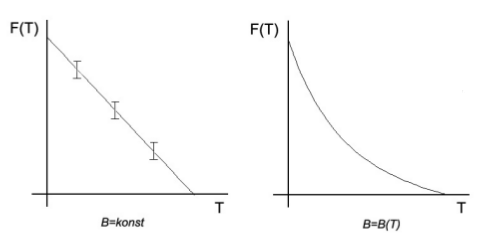
\includegraphics[width=0.6\textwidth]{subatom-08-Curie.png}
\centering
\caption{Fermiho-Curie plot.}
\label{sf8:fig:Curie}
\end{figure}

Lineárna závislosť Fermi-Curie grafu spočíva na predpoklade nulovej hmotnosti neutrína. Ak by sme uvažovali hmotnosť neutrína, tak by sa nám táto rovná čiara na konci spektra ohla smerom dolu.

Veličinu $B$, ktorá charakterizuje vplyv štruktúry atómového jadra na beta rozpad a mení sa od jadra k jadru vďaka rôzne atómové štruktúre, možno vyjadriť vzťahom
$$ B= \frac{\ln2}{fT_{1/2}},$$
kde $fT_{1/2}$ nazývame zrovnávací polčas.

\section{Rozpad $\gamma$}
Lúče $\gamma$ sú elektromagnetickou radiáciou energie, ktorá je vo všeobecnosti vyššia než $0.1\,\unit{MeV}$. Tieto lúče sú emitované pri prechode excitovaného jadra na nižšiu energetickú hladinu alebo priamo do základného stavu. Excitované jadrá obyčajne najprv prechádzajú do nižších stavov emisiou častíc a až potom nastáva gama emisia, ak je však emisia častice zakázaná výberovými pravidlami alebo obmedzená Coulombovskou bariérou tak nastáva táto gama emisia ako prvá. Ak je však možná emisia častice, tak je uprednostnená. Ku gama rozpadu dôjde, pokiaľ energia prechodu nie je dostatočne veľká na emisiu častice. Môžme teda povedať, že radiačné prechody bežne sprevádzajú beta a alfa rádioaktívne rozpady. Schematicky možno rozpad gama rozpad zapísať
$$ ^A_ZX^{*} \rightarrow ^A_ZX + \gamma.$$

Dominanciu časticovej emisie nad gama emisiou, pre energie väčšie ako prahová energia pre emisiu častice, možno preukázať jednoduchým výpočtom. Miera emisie nukleónov, ak je energeticky povolená, je úmerná frekvencii jadrového pohybu $W_n \approx \omega \approx v/R$, kde $v$ je rýchlosť nukleónu a $R$ polomer jadra. Tento vzťah približne udáva počet nárazov nukleónu na stenu jadra za jednotku času. Energia $w$ vyžiarená za jednotku času nábojom pohybujúcim sa rovnakým spôsobom je rádovo $w = \frac{e^2}{3\pi\epsilon_0c^3}\big(\frac{v^2}{R}\big)^2.$ Potom miera emisie gama lúča s energiou $\hbar \omega = \hbar(v/R)$ je 
$$ W_{\gamma} = \frac{w}{\hbar \omega} = \frac{4}{3}\frac{1}{4\pi \epsilon_0} \frac{e^2}{\hbar c} \bigg( \frac{v}{c} \bigg)^2 \frac{v}{R} << W_n. $$

Stredné doby života jadier pre rozpad gama sa nachádzajú prevažne v intervale $(10^{-7}; 10^{-11})\,s$, čo znamená, že jadrá v excitovanom stave, ktoré vznikli po rozpade alfa alebo beta, sa spravidla veľmi rýchlo dostanú do základného stavu radiačným gama prechodom. Pre tieto prechody platia podobne ako pre prechody v atómovom obale nejaké výberové pravidla. Možnosti niektorých prechodov sú však výberovými pravidlami silne potlačené a v takom prípade radiačný prechod, ktorý je dovolený z energetického hľadiska, nastáva s malou pravdepodobnosťou. Jadro môže potom pomerne dlhú dobu stráviť v niektorom excitovanom stave, jeho stav sa tak stáva metastabilným a jadro v tomto stave sa nazýva izomérom.

Jedným z typických príkladov izoméru je indium $^{115m}_{49}$In, ktorého najnižšie energetické hladiny sú na nasledujúcom obrázku \ref{sf8:fig:izomer} uvedené aj so svojimi charakteristikami - spinom a paritou. Základný stav má spin a paritu rovné $\frac{9}{2}^+$. Prvý excitovaný stav má spin a paritu rovné $\frac{1}{2}^-$ a od základného stavu sa líši neveľkou energiou $0,335\,\unit{MeV}$. Pri naznačenom prechode medzi oboma stavmi musí dôjsť k veľkej zmene momentu hybnosti (spinu) jadra a relatívne malej zmene energie. Preto je tento prechod veľmi nepravdepodobný. Stredná doba života izoméru $^{115m}_{49}$In v stave $\frac{1}{2}^-$ je 14,4 hodiny, čo je veličina o mnoho rádov väčšia než v obvyklom prípade radiačného prechodu gama. Oblasti izomerických jadier sa nachádzajú pred magickými číslami 50, 82 a 126 a v ich blízkom okolí.

\begin{figure}[!h]
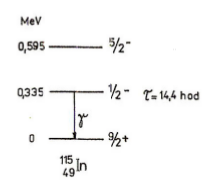
\includegraphics[width=0.4\textwidth]{subatom-08-izomer.png}
\centering
\caption{Najnižšie energetické hladiny izoméru $^{115m}_{49}In$ a nuklidu $^{115}_{49}In$.}
\label{sf8:fig:izomer}
\end{figure}

\section{Energetika $\gamma$ rozpadu}
Keď jadro prechádza z počiatočného stavu $E_i$ do koncového stavu $E_f$ je vyžiarené kvantum $\gamma$ s energiou $E_{\gamma}$, ktorá súvisí s rozdielom energii medzi oboma stavmi  $\Delta E = E_i - E_f$. Táto energia sa rozdelí medzi emitované $\gamma$ kvantum a spätný ráz jadra. Použitím zákona zachovania energie a hybnosti dostaneme vzťah
$$ \Delta E = E_{\gamma} + \frac{E^2_{\gamma}}{2Mc^2}, $$
kde $M$ je pokojová hmotnosť jadra. Keďže $E_{\gamma} \ll Mc^2$, $(\Delta E)^2 \approx E^2_{\gamma}$, vzťah sa redukuje na 
$$ E_{\gamma} \approx \Delta E - \frac{(\Delta E)^2}{2Mc^2}. $$

Odtiaľ možno nahliadnuť, že pre $A \approx 100$ je rozdiel $\Delta E$ a $E_{\gamma}$ (aj pre veľmi energetické gama žiarenie, kedy $E_{\gamma} = 10\,\unit{MeV}$) oveľa menší ako nepresnosť v meraní energie gama, ktorá činí $1$ - $2\,\unit{keV}$. Preto je možné zanedbať energiu spätného rázu jadra pri bežných meraniach gama žiarenia. Rozdiel energii medzi $\Delta E$ a $E_{\gamma}$ však hrá dôležitú úlohu v Mössbauerovom jave, ktorý má v sekcii Jadrová spektroskopia svoju vlastnú kapitolu.

Čo je tiež u gama rozpadu dôležité, je to, že vyžarovanie kvánt gama nevedie narozdiel od predchádzajúcich rozpadov ani ku zmene počtu neutrónov, ani ku zmene počtu protónov, teda ani ku zmene prvku, ani ku zmene izotopického stavu. Naviac energetické spektrum týchto fotónov je diskrétne, pretože sa jedná o prechody medzi diskrétnymi energetickými hladinami počiatočného stavu jadra o energii $E_i$ a konečného stavu jadra o energii $E_f$. Máme tu teda úplnú analógiu k tomu, čo sa odohráva pri radiačných prechodoch v obale atómu. Preto môžeme povedať, že čiarové spektrum žiarenia gama svedčí o existencii diskrétneho energetického stavu jadra.

Môžeme navyše očakávať (na základe Heisenbergovho princípu neurčitosti), že energia vznikajúcich fotónov pri radiačných prechodoch v jadre bude podstatne väčšia ako energia fotónov vyžarovaných z atómového obalu.

Energetické spektrum gama žiarenia je vyobrazené na obrázku \ref{sf8:fig:gama}. Jedná sa o spektrum, ktoré spája spojité spektrum elektrónov emitovaných pri beta rozpade, na ktoré sú nanesené ostré piky Augerových a konverzných elektrónov pochádzajúcich z gama prechodov.

\begin{figure}[!h]
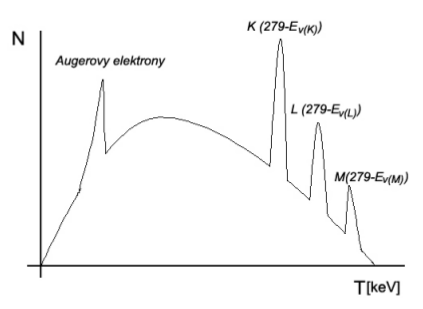
\includegraphics[width=0.6\textwidth]{subatom-08-gama.png}
\centering
\caption{Energetické spektrum gama žiarenia.}
\label{sf8:fig:gama}
\end{figure}

\section{Výberove pravidla}
Emisia gama je formou elektromagnetického žiarenia a ako taká je spôsobená zmenou elektrického poľa indukujúceho magnetické pole. Rozoznávame dva druhy emisie gama - elektrické (E) vyžarovanie a magnetické (M) vyžarovanie. Tieto názvy pochádzajú zo semiklasickej teórie žiarenia, v ktorej žiarenie vzniká v dôsledku časovej zmeny rozdelenia prúdu a náboja. Klasifikácia výsledného žiarenia je založená na fakte, že celkový moment hybnosti rovnako ako parita (jedná sa o elektromagnetický prechod) sa zachovávajú.

Fotón si odnáša celkový moment hybnosti, daný kvantovým číslom $J$, ktorý musí rešpektovať fakt, že fotón je vektorový bozón so spinom rovným jednej. Minimálna hodnota je tak $J=1$, pretože reálny fotón má dva možné stavy polarizácie zodpovedajúce napríklad $J_z=\pm 1$. Ak označíme spin jadra v počiatočnom stave $J_i$ a spin jadra v koncovom stave $J_f$, vidíme, že prechod $J_i=0 \rightarrow J_f=0$ je striktne zakázaný.

Fotóny majú všeobecne multipolaritu $J$, a tak môžme rozlišovať aj multipolaritu prechodov, ktorá môže byť dipólová ($J = 1$), kvadrupólová ($J = 2$), oktupólová ($J = 3$) atď.

Pre celkový moment musí platiť
$$ \vec{J} = \vec{J}_i - \vec{J}_f $$
$$ \vert J_i - J_f \vert \leq J \leq J_i + J_f. $$

Dôležité je vziať do úvahy tiež paritu. V klasickej fyzike je dipól $q\vec{r}$ sformovaný ako dva opačné náboje $q$ vo vzdialenosti $\vec{r}$. Zmenou $\vec{r} \rightarrow -\vec{r}$ zistíme, že má zápornú paritu. Magnetický dipól je ekvivalentný nábojom cirkulujúcim rýchlosťou $\vec{v}$ a formujúcim tak prúdovú slučku polomeru $r$. Magnetický dipól tak má tvar $q\vec{r} \times \vec{v}$, čo nemení znamienko pri inverzii parity, a má tak kladnú paritu. Všeobecne platí, že elektricky multipólový prechod má paritu $(-1)^L$, zatiaľčo magnetický multipólový prechod má paritu $(-1)^{L+1}$. Výberové pravidla pre gama emisiu máme zhrnuté v nasledujúcej tabuľke
\begin{figure}[!h]
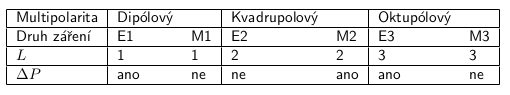
\includegraphics[width=0.7\textwidth]{subatom-08-pravidla.png}
\centering
\end{figure}

Hoci sú prechody $J_i = 0 \rightarrow J_f = 0$ zakázané kvôli tomu, že fotón je reálna častica, v prípade, že by bol fotón virtuálny, sa takéto prechody môžu prihodiť (parita sa pritom nemení). Dôvodom pre to je skutočnosť, že polarizačné stavy virtuálneho fotónu nie sú obmedzené tak ako polarizačné stavy reálneho fotónu. Energia virtuálneho fotónu sa môže odovzdať atómovému elektrónu, ktorý je tak emitovaný z atómu. Ide pritom zvyčajne o elektrón z niektorej z vnútorných vrstiev, teda K alebo L, ktorého vlnová funkcia presahuje do jadra. Tento proces sa nazýva vnútorná konverzia.

\section{Vnútorná konverzia elektrónov}
Vyššie sme spomenuli že elektromagnetický prechod medzi dvoma excitovaným stavmi sa môže prihodiť aj prostredníctvom vnútornej konverzie. K tomuto javu dochádza z dôvodu interakcie jadrového elektromagnetického poľa s atómovým elektrónom, ktorému tak odovzdáva dostatočnú energiu na opustenie atómu. Elektrón je emitovaný s diskrétnou energiou, ktorá je spojená s rozdielom $\Delta E = E_i - E_f$ medzi dvoma stavmi, vzťahom
$$ E_e = \Delta E - B_e - T_R ,$$
kde $B_c$ je väzbová energia elektrónu a $T_R$ je energia spätného rázu jadra.

Emitované elektróny pochádzajú z rôznych orbitálov, teda obvykle pozorujeme niekoľko diskrétnych línii vnútornej konverzie, tj. energetické spektrum elektrónov vyžiarených pri vnútornej konverzii je čiarové. Pravdepodobnosť vnútornej konverzie pre rôzne atómy a excitované hladiny je rôzna a charakterizuje sa tzv. konverzným koeficientom, ktorý udáva pomer stredného počtu procesov $N_e$ (vyžiari sa elektrón), ku strednému počtu procesov $N_{\gamma}$ (vyžiari sa gama). Konverzný koeficient tiež silne závisí na rozdiely $\Delta E$, protónovom čísle $Z$ a na vrstve. Je daný vzťahom
$$ \alpha_k = \frac{N_e}{N_{\gamma}}. $$

Typický prípad, v ktorom nastáva vnútorná konverzia, je demonštrovaný na obrázku \ref{sf8:fig:konverzia}. Majme izotop germánia $_{32}^{72}$Ge, ktorého základný a prvý excitovaný stav majú rovnaký spin rovný nule a párnu paritu. Zákon zachovania momentu hybnosti nedovoľuje, aby došlo medzi týmito stavmi k radiačnému prechodu, pretože fotón má spin rovný jednej. Pri deexcitáci, ktorá sa tu často označuje ako $0-0$ prechod, odovzdá jadro germánia elektrónu energiu $0,69\,\unit{MeV}$ a ten nadobudne kinetickú energiu podľa vyššie uvedeného vzťahu.

\begin{figure}[!h]
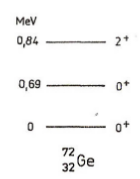
\includegraphics[width=0.2\textwidth]{subatom-08-konverzia.png}
\centering
\caption{Najnižšie energetické hladiny jadra $_{32}^{72}Ge$.}
\label{sf8:fig:konverzia}
\end{figure}

Ak je vzdialenosť medzi hladinami daného nuklidu väčšia ako $2m_ec^2$, kde $m_e$ je pokojová hmotnosť elektrónu, a ak nie je medzi týmito hladinami dovolený radiačný prechod, môže jadro prejsť do nižšieho energetického stavu aj tak, že sa v jeho elektromagnetickom poli vytvorí pár pozitrón a elektrón, ktorý odnesie príslušnú energiu. Tento jav, ktorý možno pozorovať napríklad pri deexcitaci kyslíka $_{8}^{16}$Ge, je nazývaný dvojitou konverziou. U uvedeného jadra je to opäť $0-0$ prechod, pri ktorom sa znižuje energia jadra o $6,1\,\unit{MeV}$. Na dvojitej konverzii sa nepodieľa elektrónový obal. 

Vnútorná konverzia často sprevádza beta rozpad, pretože materské jadrá môžu prechádzať beta rozpadom na dcérske jadra v excitovanom stave, ktoré sa ďalej deexcitujú práve elektromagnetickými prechodmi. Vďaka tomu často v energetickom spektre beta žiarenia pozorujeme sadu diskrétnych čiar. 

Ešte spomeňme, že pomenovanie tohto javu pochádza z historického označenia vnútorná konverzia žiarenia gama, ktoré vzniklo na základe mylnej domnienky, že k emisii elektrónov dochádza v dôsledku absorpcie fotónu gama, ktorý je emitovaný jadrom v atómovom obale. V skutočnosti ale fotón žiarenia gama z jadra nevyletí (je len virtuálny), energia deexcitácie vzbudenej hladiny jadra je odovzdaná najbližšiemu elektrónu (teda elektrónu na najnižšej vrstve - K vrstve) priamo.

\section{Jadrový izomér}
Väčšina jadrových excitovaných stavov je veľmi nestabilná a prakticky okamžite deexcituje vyžiarením fotónového žiarenia gama. V niektorých prípadoch však jadrové excitované hladiny nedeexcitujú okamžite, ale až po uplynutí určitého dlhšieho času - hovoríme, že sú metastabilné. Tento jav sa tiež nazýva jadrová izoméria. 

\paragraph{Príčina metastability a izomérie} 
Hlavným mechanizmom potlačenia gama deexcitácie vzbudených jadrových hladín, ktorému metastabilné izoméry vďačia za svoje dlhé polčasy, je relatívny zákaz gama prechodu z dôvodu veľkého rozdielu momentov hybnosti (spinov) medzi príslušnými jadrovými hladinami - spinový nesúlad. 

\paragraph{Vnútorná konverzia žiarenia gama a X, konverzné a Augerové elektróny}
Pokiaľ je jadro súčasťou atómu, nemusia sa všetky deexcitácie v jadre vyžiariť ako fotóny žiarenia gama. Môže dôjsť ku konkurenčným procesom, zabraňujúcim emisii fotónov žiarenia gama pri deexcitácii vzbudených jadrových hladín - predovšetkým k procesu tzv. vnútornej elektrónovej konverzie žiarenia gama. Energia jadrovej deexcitácie sa nevyžiari, ale je predaná niektorému elektrónu v obale, ktorý potom vylieta ako tzv. konverzný elektrón.

\begin{figure}[!h]
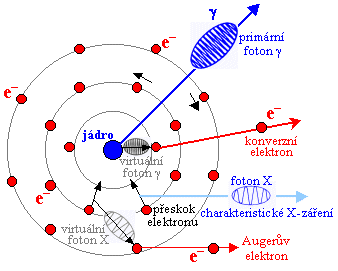
\includegraphics[width=0.5\textwidth]{subatom-08-izometria.png}
\centering
\caption{Schematické znázornenie vnútornej konverzie žiarenia gama za vzniku konverzných elektrónov a charakteristického X-žiarenia a vnútornej konverzie žiarenia X za vzniku Augerových elektrónov.}
\label{sf8:fig:izometria}
\end{figure}

Na obrázku \ref{sf8:fig:izometria} sú schematicky znázornené všetky príslušné procesy. Predovšetkým, modrou šípkou je znázornený základný prípad nerušeného vyžiarenia fotónu gama z excitovaného jadra. Proces vnútornej konverzie si môžme zjednodušene predstaviť tak, že fotón gama, emitovaný pri deexcitácii sa môže zraziť s obalovým elektrónom vlastného atómu, ktorý preberie celú jeho energiu (dôjde k fotoefektu), fotón gama zanikne a miesto neho vyletí elektron uvoľnený vďaka prijatej energii. Tento jav je bežne pozorovaný, nazýva sa vnútorná konverzia žiarenia gama (alebo vnútorný fotoefekt) a príslušné elektróny sa nazývajú konverzné elektróny.

Uvedený mechanizmus vnútornej konverzie je potrebné považovať len za heuristický prístup. Fotón žiarenia gama v skutočnosti vôbec z jadra nevyletí (je jen virtuálny), takže energia deexcitácie je elektromagnetickou interakciou predaná najbližšiemu obalovému elektrónu priamo a ten potom z atómu vyletí s kinetickou energií danou rozdielom energie deexcitácie jadra a väzbovej energie elektrónu v obale. Fyzické vyžiarenie fotónu gama nie je nutné, keďže vlnová funkcia obalových elektrónov čiastočne preniká do jadra (je nenulová pravdepodobnosť výskytu elektrónu v oblasti jadra) a interakcia môže nastať bezprostredne. Navzdory svojmu názvu tak vnútorná konverzia nie je dvojstupňový proces (pri ktorom by se fotón gama najprv emitoval a potom bol pohltený elektrónom, ktorý sa vyžiari), ale priamym jednostupňovým elektromagnetickým procesom.

\section{Transuránové prvky}
Sú prvky, ktoré nasledujú v Mendelejevovej periodickej sústave za uránom. V prírode sa bežne nevyskytujú, všetky sa pripravujú umelo. Ľahšie transurány, ako je neptúnium, plutónium, amerícium a curium, sú produkované v ľahkovodných jadrových reaktoroch. Majú pomerne dlhé polčasy rozpadu a možno ich teda extrahovať z vyhoreného jadrového paliva chemickou cestou.

\paragraph{Príprava}
Východiskový materiál pre prípravu všetkých transuránov je urán-238, najťažší nuklid, ktorý sa vyskytuje v prírode. Používajú sa dve metódy prípravy ťažkých prvkov:
\begin{itemize}
\item Záchyt niekoľkých neutrónov a následný beta rozpad vzniknutého izotopu.
\item Bombardovanie ťažkých prvkov urýchlenými iónmi, napr.:$$ ^{238}_{92}U (d,2n) ^{238}_{93}Np $$
Bombardovaním ľahkými časticami (deuteróny, alfa častice) získame prvky s atómovým číslom vyšším o jednu až dve jednotky, ak ale použijeme ťažšie ióny, napr. uhlík-12 alebo kyslík-16 môžme získať prvky s protónovým číslom vyšším o šesť až desať jednotiek oproti východiskovému jadru.

\end{itemize}

\end{document}